%\setlength{\textwidth}{5.5in}
%\documentstyle[12pt]{article} 
%\setlength{\textwidth}{5.5in}
%\setlength{\textheight}{8.0in} %\setlength{\baselineskip}{12pt}
%\pagestyle{headings}

%% Remove line numbering for arXiv submission
%\RequirePackage{lineno}
%\setlength{\linenumbersep}{6pt}
%\linenumbers

\documentclass[12pt,letterpaper,aps,prc,superscriptaddress,showpacs,
longbibliography,nofootinbib,floatfix,onecolumn]{revtex4-1}

\setlength{\textwidth}{6.5in}
%\documentstyle[12pt]{article}
\setlength{\textheight}{9.5in}


%\usepackage{hyperref}
\usepackage{graphicx}
\usepackage{dcolumn}

\usepackage{xspace}
\usepackage{color}
                 
% GENERAL DEFINITIONS 
 
\newcommand\ie {{\it i.e. }} 
\newcommand\vs {{\it vs }} 
\newcommand\eg {{\it e.g. }}
\newcommand\etc{{\it etc. }} 
\newcommand\cf {{\it cf.  }}
%\newcommand\pt {$p_{\rm T}$}
%\newcommand\gevc {GeV/$c$}
\newcommand\grad{\nabla} 
\newcommand\as{$\alpha_s$}
\newcommand\aem{$\alpha_{em}$}


\newcommand{\red}{\textcolor{red}}
\newcommand{\blue}{\textcolor{blue}}
\newcommand{\green}{\textcolor{green}}
\newcommand{\taa}{\mbox{$T_{\rm AA}$}\xspace}
\newcommand{\TAB}{\mbox{$T_{\rm AB}$}\xspace}
\newcommand{\Teff}{\mbox{$T_{\rm eff}$}\xspace}
\newcommand{\pt}{\mbox{$p_{\rm T}$}\xspace}
\newcommand{\kt}{\mbox{$k_{\rm T}$}\xspace}
\newcommand{\mt}{\mbox{$m_{\rm T}$}\xspace}
\newcommand{\ptg}{\mbox{$p_{\rm T}$}^{\gamma}$\xspace}
\newcommand{\raa}{\mbox{$R_{\rm AA}$}\xspace}
\newcommand{\rab}{\mbox{$R_{\rm AB}$}\xspace}
\newcommand{\raap}{\mbox{$R_{\rm AA}^{N_{\rm part}}$}\xspace}
\newcommand{\rda}{\mbox{$R_{\rm dA}$}\xspace}
\newcommand{\Npart}{\mbox{$N_{\rm part}$}\xspace}
\newcommand{\Ncoll}{\mbox{$N_{\rm coll}$}\xspace}
\newcommand{\Nqp}{\mbox{$N_{\rm qp}$}\xspace}
\newcommand{\Nch}{\mbox{$N_{\rm ch}$}\xspace}
\newcommand{\dNdeta}{\mbox{$dN_{\rm ch}/d\eta$}\xspace}
\newcommand{\ebj}{\mbox{$\varepsilon_{\rm BJ}$}\xspace}
\newcommand{\Et}{\mbox{$E_{\rm T}$}\xspace}
\newcommand{\xt}{\mbox{$x_{\rm T}$}\xspace}
\newcommand{\meanz}{\mbox{$\langle z \rangle$}\xspace}
\newcommand{\meanpt}{\mbox{$\langle p_{\rm T} \rangle$}\xspace}
\newcommand{\meanet}{\mbox{$\langle E_{\rm T} \rangle$}\xspace}
\newcommand{\sqs}{\mbox{$\sqrt{s}$}\xspace}
\newcommand{\sqsn}{\mbox{$\sqrt{s_{_{NN}}}$}\xspace}
\newcommand{\snn}{\mbox{$\sqrt{s_{_{NN}}}$}\xspace}
\newcommand{\sqsntwo}{\mbox{$\sqrt{s_{_{NN}}}=200$~GeV}\xspace}
\newcommand{\NN}{\mbox{$NN$}\xspace}
%\newcommand{\pp}{\mbox{$p$$+$$p$}\xspace}
%\newcommand{\pn}{\mbox{$p$$+$$n$}\xspace}
%\newcommand{\nn}{\mbox{$n$$+$$n$}\xspace}
\newcommand{\pp}{\mbox{$pp$}\xspace}
\newcommand{\pbarp}{\mbox{$p\bar{p}$}\xspace}
\newcommand{\pn}{\mbox{$pn$}\xspace}
\newcommand{\nn}{\mbox{$nn$}\xspace}
\renewcommand{\AA}{\mbox{A$+$A}\xspace}
\newcommand{\AB}{\mbox{A$+$B}\xspace}
\newcommand{\pA}{\mbox{p$+$A}\xspace}
\newcommand{\dau}{\mbox{$d$$+$Au}\xspace}
\newcommand{\pdau}{\mbox{$p(d)$$+$Au}\xspace}
\newcommand{\pau}{\mbox{$p$$+$Au}\xspace}
\newcommand{\auau}{\mbox{Au$+$Au}\xspace}
\newcommand{\cucu}{\mbox{Cu$+$Cu}\xspace}
\newcommand{\cuau}{\mbox{Cu$+$Au}\xspace}
\newcommand{\pbpb}{\mbox{Pb$+$Pb}\xspace}
\newcommand{\uu}{\mbox{U$+$U}\xspace}
\newcommand{\jpsi}{\mbox{$J/\psi$}\xspace}
\newcommand{\Etemc}{\mbox{${\rm{E}}_{T\,{\rm EMC}}$}\xspace}
\newcommand{\sloss}{\mbox{$S_{\rm loss}$}\xspace}
\newcommand{\piz}{\mbox{$\pi^0$}\xspace}
\newcommand{\dptpt}{\mbox{$\delta p_{\rm T}/p_{\rm T}$}\xspace}
\newcommand{\dnchdeta}{\mbox{$dN_{\rm ch}/d\eta$}\xspace}
\newcommand{\dngamdeta}{\mbox{$dN_{\gamma}/d\eta$}\xspace}
\newcommand{\ptpp}{\mbox{$p_{\rm T}^{pp}$}\xspace}
\newcommand{\vtwo}{\mbox{$v_2$}\xspace}
\newcommand{\vthr}{\mbox{$v_3$}\xspace}
\newcommand{\rgam}{\mbox{$R_{\gamma}$}\xspace}
\newcommand{\mgg}{\mbox{$m_{\gamma\gamma}$}\xspace}
\newcommand{\mee}{\mbox{$m_{e^{+}e^{-}}$}\xspace}
\newcommand{\meeg}{\mbox{$m_{e^{+}e^{-}\gamma}$}\xspace}
\newcommand{\gam}{\mbox{$\gamma$}\xspace}
\newcommand{\gev}{\mbox{GeV}\xspace}
\newcommand{\gevc}{\mbox{GeV/$c$}\xspace}
\newcommand{\fmc}{\mbox{fm/$c$}\xspace}



 
\def\be{\begin{equation}}
\def\ee{\end{equation}}  

%\input epsf
\renewcommand{\topfraction}{0.9} 
\renewcommand{\bottomfraction}{0.9} 
\renewcommand{\textfraction}{0.1} 
\renewcommand{\floatpagefraction}{0.80} 
 
\begin{document} 

\begin{center}
{\bf Neutral meson and photon ntuples \\ 
 explanation, and examples}
\end{center}

\vspace{0.2in}

\begin{center}
{\it Gabor David \\
Stony Brook University, Brookhaven National Laboratory}
\end{center}

\vspace{0.3in}



% Delete this at the end
%\tableofcontents

%\newpage

%\vspace{0.2in}

%\section{\bf Purpose, technology, dimensions}
%\label{sec:purpose}

{\bf $\pi^0$-s and photons ($\gamma$-s)} \\
\vspace{0.05in}

\noindent
Based on real data this write-up introduces you how to find $\pi^0$-s
and photons in an electromagnetic calorimeter (EMcal).  They contain
information on {\it clusters} -- small, contiguous regions of energy
deposit in the EMCal -- which are usually considered as 
{\it energy deposited by one single particle}.  While this is not
always true, this is our first working hypothesis, but we should
always be aware that a cluster might contain energy from more than one
particle.  Also, not all
clusters correspond to photons; many are from hadrons, especially at
low and very high \pt (transverse momentum)\footnote{This may sound
  surprising in an electromagnetic calorimeter, but it is true: many
  high \pt single clusters are actually from two overlapping photons
  from a \piz decay, i.e. they are hadrons.
}.  
In fact, it's going to
be your job to find selection criteria (``cuts'') which eliminate
hadrons (the {\it contamination}) but still preserves most of the
photons ({\it signal}) in the sample.

As for \piz, recall that most of them decay via 
$\pi^0 \rightarrow \gamma\gamma$, so they can be reconstructed from
photon candidate {\it pairs} using the invariant mass
$$ m_{\gamma\gamma} = \sqrt{2E_1E_2(1-cos(\theta))} $$
where $E_1,E_2$ are the energies of the two photon candidates and
$\theta$ is the {\it opening angle} between them.  Note that the \pt
of the \piz is simply the vector sum of the \pt-s of the two photons
paired. 

Please note that -- as per PHENIX standards -- time is always given in
nanoseconds, distance in centimeters and energy in GeV.


\vspace{0.1in}
{\bf The {\it gnt} and {\it ggntuple} Ntuples} \\
\vspace{0.05in}

\noindent
The two files {\it MBntup.root} and {\it ERTntup.root} are produced
using a small fraction of the \sqsn=200\,GeV $p$+Au data collected by
PHENIX in 2015.  They are published for educational purposes only.
You will not be able to derive any publishable physics results from
them, however, you can learn some basic techniques of
particle identification (PID), practice how to make different cuts and
estimate their effect, how the signal to background ratio can be
improved at the expense of some loss in the signal and how to find an
optimum between the two trends.  You may also learn that PID itself is
also not an unambiguous procedure: you can apply much looser cuts on
the ``photonness'' of the clusters when reconstructing \piz, because
you identify the \piz by the {\it correlation} of the two ``photons'',
namely, whether their invariant mass is in the expected range (around
0.135\,\gev) or not.  Only photon pairs from the decay of the same
\piz are truly correlated, random pairs of photons, photon-hadron or
hadron-hadron pairs only rarely give invariant masses in the 
``\piz window''.  Therefore, you can allow yourself to have more
contamination is the ``photon'' sample -- and gain significant
statistics in reconstructed \piz (why?).  --  On the other hand for
reconstructing (inclusive) photons you don't have such a help: if you
decide that a cluster is a photon, that's it.  In order to keep the
contamination from misclassified hadrons you might want to make your
photon PID cuts stricter, in order to increase {\it purity} 
(in other terminology decrease {\it contamination}) at the
expense of {\it efficiency}.

\vspace{0.05in}
\noindent
The first Ntuple is called {\it ggntuple} (gamma-gamma ntuple) and
contains information on EMCal cluster {\it pairs} and the two clusters
in the pair (see Table~\ref{tab:ggntuple}).  In each event all
clusters in a sector are paired with all other clusters, and the pair
variables ({\it pt, costheta, phi, mass, asym}) calculated, even if
they are obviously not photons from a \piz decay (for instance because
their invariant mass is, say, 0.4\,\gev).  These ``obviously wrong''
random pairs are called the {\it combinatorial background} and they
help you to estimate the background in the \piz peak when you'll try
to extract the number of \piz in the sample.
The momenta attributed to a cluster (particle candidate) is calculated
from the vector connecting the collision point ({\it vtxZ}) with the
impact point on the EMCal, and under the assumption that the particle
is a photon (i.e. $p=E$, the measured energy).  From these, the pair
momentum {\it pt} is calculated as the vector sum of the transverse
components; {\it costheta} is the cosine of the opening angle between
the two momentum vectors, {\it phi} is the azimuth of the pair
momentum (i.e. of the parent \piz), {\it mass} is the invariant mass
calculated with the formula above, and {\it asym} is the energy
asymmetry $\alpha$ of the two clusters
$$\alpha = \frac{|E_1-E_2|}{E_1+E_2}$$
The rest of the variables describe the two clusters ({\it 1,2}), their
meaning is spelled out below.


\begin{table}[h]
  \begin{tabular}{|l|l|} \hline
    Variable name & Description \\ \hline
    cent & Event centrality \\
    vtxZ & $z$-vertex of the event \\
    pt   & Transverse momentum of cluster {\it pair} ($\pi^0$
    candidate) \\
    costheta & $cos$ of the opening angle between the two clusters \\    
    phi & Azimuthal angle of the direction of the pair momentum
    (assumed $\pi^0$) \\
    mass & Invariant mass calculated from the two clusters (energy and
    position) \\
    asym & Energy asymmetry ($|E_1-E_2|/(E_1+E_2)$) of the two clusters \\
    sec1 & EMCal sector where the first cluster is \\
    Ecore1 & ``Core'' energy of the first cluster \\
    tof1   & Time-of-flight of the first cluster \\
    twrhit1 & Number of towers in the first cluster \\
    prob1 & Probability that the first cluster is a photon (based on
    $\chi^2$) \\
    chisq1 & $\chi^2$ from expected photon shape for the first cluster
    \\
    stoch1 & Combined variable to describe ``photonness'' of first
    cluster \\
    sec2 & ...  Same quantities as above for the second cluster of the
    pair \\ \hline
  \end{tabular}
  \vspace{0.3cm}
  \caption{Fields in the $\gamma$-pair Ntuple ({\it ggntuple}).
}
  \label{tab:ggntuple}
 \end{table}

\vspace{0.05in}
\noindent
The second Ntuple is called {\it gnt} and contains information on
individual clusters (again, many of which are {\it not} photons!).
Here {\it pt} is the transverse momentum of the (single) particle,
calculated under the assumption that it is a photon (straight path
from the collision vertex and $p=E$), {\it costheta} is the cosine of
the polar angle, {\it phi} is the azimuth, and {\it sec} is the sector
number (0-5 are lead scintillator sectors, PbSc, 6-7 are lead glass,
PbGl).  For both detectors the smallest, individually read out units
are called {\it towers}.

\noindent
The field {\it ecore} is an estimate of the particle energy (using various
corrections to account for detector effects), {\it ecent} is the
energy in the central (highest energy) tower of the cluster, 
{\it tof} is the time-of-flight measured in the central tower and
corrected with the flight-path $s/c$ such that for photons {\it tof}
is a distribution around zero.  Based on testbeam data we have a model
(parametrization) of electromagnetic showers depending on energy, impact
point and angle of the photon; the {\it chisq} is calculated as the
deviation of the actual shower (energy deposit pattern in the towers)
from the ``model'' shower of the same energy, impact point and angle.
The {\it prob} is calculated from this $\chi^2$, usually showers with
$prob>0.05$ are very likely indeed photons;  {\it disp} is the 2D
dispersion, {\it twrhit} is the number of towers hit (i.e. included in
the cluster), finally {\it stoch} is a combination of various
probability measures to characterize ``photonness'', higher values
mean higher probability that the cluster is indeed a photon.  The
calculated impact point of the particle is given as $x,y,z$ in the
PHENIX absolute coordinate system ($x>0$ is the West Arm, negative $z$
is South).

The {\it MBntup.root} file is produced from minimum bias data (although
with a lower limit  \pt$>2.0$\,\gevc in {\it gnt} and pair \pt in
{\it ggntuple}), whereas in {\it ERTntup.root} the threshold for 
single cluster \pt in {\it gnt} is 8\,\gev, and the threshold for pair
\pt in {\it ggntuple} is also 8\,\gev.  Note that since here we
restrict only the pair \pt, the energy of the individual clusters can
be (and often is) significantly lower.  Important: both the MB and the
ERT {\it ggntuple}-s are written out with the condition that the
asymmetry is less than 0.8.

\begin{table}[h]
  \begin{tabular}{|l|l|} \hline
    Variable name & Description \\ \hline
    cent & Event centrality \\
    vtxZ & $z$-vertex of the event \\
    pt   & Transverse momentum of the cluster ($\gamma$-candidate) \\
    costheta & Polar angle of the cluster ($\gamma$-candidate) \\    
    phi & Azimuthal angle of the cluster ($\gamma$-candidate) \\
    sec & EMCal sector of the cluster ($\gamma$-candidate) \\
    ecore & ``Core'' energy of the cluster ($\gamma$-candidate) \\
    ecent & Energy in the central tower of the cluster ($\gamma$-candidate) \\
    tof   & Time-of-flight in the central tower of the cluster ($\gamma$-candidate) \\
    prob & Probability that the cluster is a photon (based on $\chi^2$) \\
    disp & Dispersion of the cluster ($\gamma$-candidate) \\
    chisq & $\chi^2$ from expected photon shape of the cluster ($\gamma$-candidate) \\
    twrhit & Number of towers in the cluster ($\gamma$-candidate) \\
    stoch & Combined variable to describe ``photonness'' of the cluster ($\gamma$-candidate) \\
    x & $x$-position of impact point on the EMCal surface \\
    y & $y$-position of impact point on the EMCal surface \\
    z & $z$-position of impact point on the EMCal surface \\ \hline
  \end{tabular}
  \vspace{0.3cm}
  \caption{Fields in the $\gamma$ Ntuple ({\it gnt}).
}
  \label{tab:gnt}
 \end{table}

\newpage
%\vspace{0.1in}
{\bf Examples} \\
\vspace{0.05in}

\noindent
Here are a few simple example plots illustrating what you can do,
based on the MB and ERT (high \pt) data.  (The amount of data, i.e. the
statistics might be different in the released datafiles, but you
should be able to reproduce the overall features of the histograms.)

\noindent
\begin{verbatim}
f1 = new TFile("MBntup.root");
f2 = new TFile("ERTntup.root");
f1->cd();
ggntuple->Draw("mass","mass<1.0");
f2->cd();
ggntuple->Draw("mass","mass<1.0");
f1->cd();
ggntuple->Draw("mass>>htemp1","mass<1.0");
ggntuple->Draw("mass>>htemp2","mass<0.4&&chisq1<3.0&&chisq2<3.0");
htemp2->SetLineColor(2);
htemp1->Draw();
htemp2->Draw("same");
\end{verbatim}
For characteristic results see Fig.~\ref{fig:invmass}.  The left panel
shows the \mgg distribution in the MB data (no cut on \pt or any
other observable).  While the true \piz peak dominates (0.135\,\gev),
there is a pronounced peak at 0.03\,\gev (primarily due to 
``minimum ionization'' hadrons),
also, the combinatorial background under the true \piz peak is
substantial.  The middle panel is the same \mgg distribution from the
ERT data.  The fake peak at 0.03\,\gevc is gone, the combinatorial
background is much smaller, and now you clearly see the peak at the
$\eta$ meson mass as well.  The right panel is once again MB data; the
blue histogram is the (uncut) \mgg (same as on the left panel), the
red is the same \mgg if we require that both clusters of the pair
satisfy the $\chi^2<3$ condition (i.e. are consistent with the photon
cluster shape).  Note the log scale.  As you can see, the cut on
``photonness'' leaves the \piz peak area nearly unchanged, but reduces
the combinatorial background drastically.

\newpage

\begin{center}
\begin{figure}[htbp]
  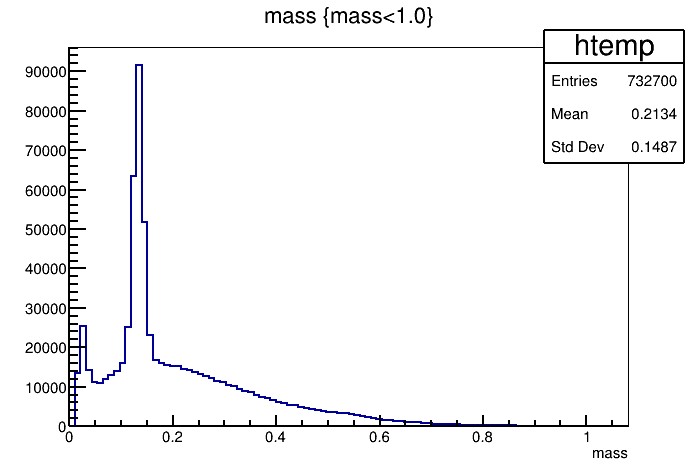
\includegraphics[width=0.3\linewidth]{figs/mbinvmass.png}
  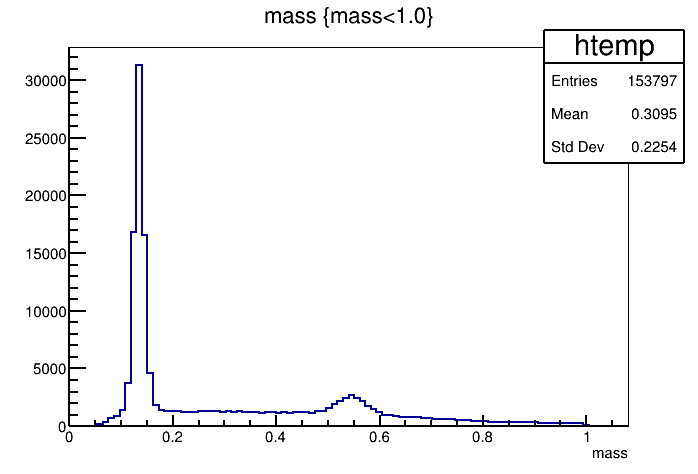
\includegraphics[width=0.3\linewidth]{figs/ertinvmass.png}
  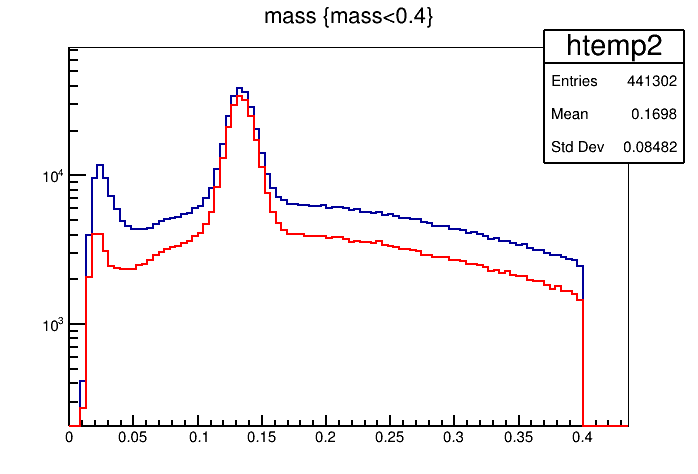
\includegraphics[width=0.3\linewidth]{figs/chi2mbinvmass.png}
  \caption{Left panel: Invariant mass from the MB data
    in the 0-1\,\gev region.  You can see a strong \piz peak
    and maybe a hint of $\eta$.
    Middle panel: \piz peak for pairs 
    from the ERT data (i.e. the pair \pt is greater than 8\,\gevc.  
    The combinatorial background is much smaller and the $\eta$ peak
    is now clearly seen.
    Right panel: the effect of a strong $\chi^2$ cut on the photon
    pairs in the MB data.  The blue histogram is the same as in the
    left panel, the red is with the $\chi^2$ cut on both clusters.
    While you barely lose any signal (due to the small inefficiency of
    the cut), the signal to background ratio improves dramatically.
  }
    \label{fig:invmass}
\end{figure}
\end{center}

The (energy) asymmetry of the two \piz decay photons is a flat
distribution by kinematics (at least in $4\pi$ solid angle).  This
offers another opportunity to improve the signal/background ratio when
extracting the \piz-s.   
In the left panel of Fig.~\ref{fig:asym_pt} the asymmetry distribution
of all \mgg pairs is shown (MB data).  The enhancement at high
asymmetries comes from the abundant low \pt photons and hadrons
depositing small energy - i.e. non-\piz, combinatorial background
pairs.  By applying a modest, say $\alpha<0.6$ asymmetry cut the S/B
ratio can be significantly improved at a small cost of lost true
\piz-s, as demonstrated in the right panel of Fig.~\ref{fig:asym_pt}. 
The ROOT commands are here:


\begin{verbatim}
ggntuple->Draw("asym","mass<1.0");
ggntuple->Draw("mass>>htemp1","mass<1.0");
ggntuple->Draw("mass>>htemp2","mass<1.0&&asym<0.6");
htemp1->Draw();
htemp2->Draw("same");
\end{verbatim}


\begin{center}
\begin{figure}[htbp]
  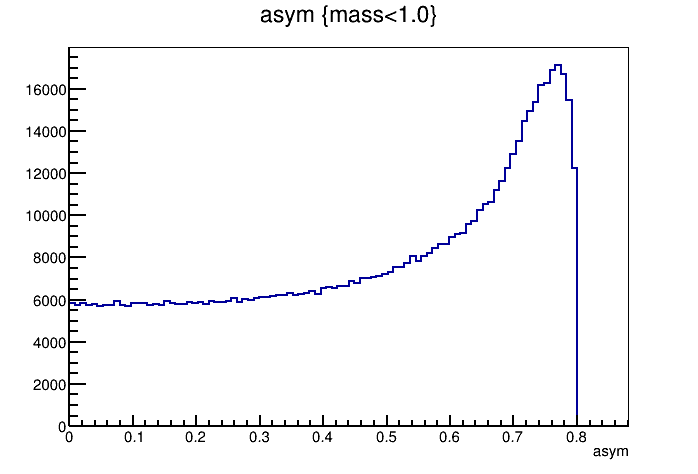
\includegraphics[width=0.4\linewidth]{figs/mbasym.png}
  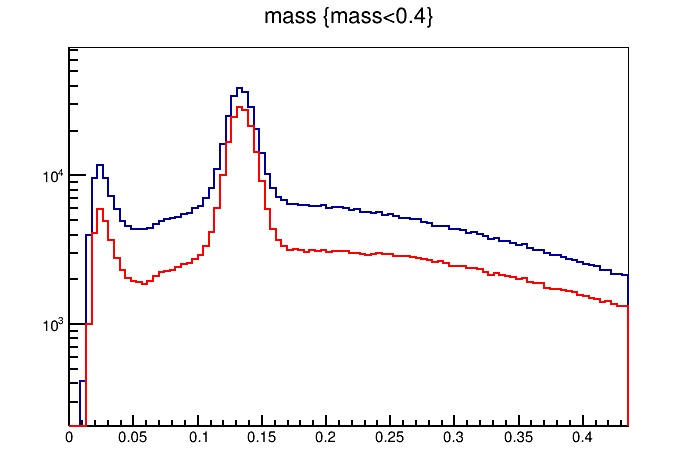
\includegraphics[width=0.4\linewidth]{figs/mbinvmassasym.png}
  \caption{MB data, plots from the pair ntuple.  Left panel: energy
    asymmetry distribution for all pairs.  
    Right panel: invariant mass distribution without asymmetry cut
    (i.e. with the default $\alpha<0.8$) and with a tighter
    $\alpha<0.6$ cut (red histogram.  The signal to combinatorial
    background ratio is significantly improved.
  }
    \label{fig:asym_pt}
\end{figure}
\end{center}

Let's make a crude estimate of the {\it raw} \piz and $\eta$ spectrum,
i.e. the pair \pt distribution of those pairs which give an invariant
mass in the \piz or $\eta$ ``mass window''.  The estimate will be
crude because we don't attempt to account for the combinatorial
background.  However, we can try to clean up the spectra by making a
cut on the ``photonness'' of both clusters.  This is illustrated in
Fig.~\ref{fig:pizeta_pt} for \piz in both MB and ERT data, and $\eta$
(ERT only).  The blue histograms are the \pt distribution of pairs in
the mass window, the red histoes the same but with an additional cut
on the {\it chisq} variables.  The principal commands:

\begin{verbatim}
ggntuple->Draw("pt","abs(mass-0.135)<0.015");
ggntuple->Draw("pt","abs(mass-0.135)<0.015&&chisq1<3.0&&chisq2<3.0");
ggntuple->Draw("pt","abs(mass-0.548)<0.1");
ggntuple->Draw("pt","abs(mass-0.548)<0.1&&chisq1<3.0&&chisq2<3.0");
\end{verbatim}

Note that the mass window for \piz is much narrower than for $\eta$.
In the MB \piz spectra at low \pt the {\it chisq} cut eliminates 
some 20-30\% of \piz counts (red vs blue histogram), in line with what
the left plot in Fig.~\ref{fig:invmass} suggests (the estimated
magnitude of the combinatorial background).  In ERT there is very
little change, again in line with the small combinatorial on the
middle panel in Fig.~\ref{fig:invmass}.  Finally, for $\eta$ there is
a significant drop in the yields for the entire (high \pt) spectrum,
in line with the large combinatorial (as compared to the small peak)
in Fig~\ref{fig:invmass}.  Also, the spurios ``flattening'' at very
high \pt in the blue histogram is completely gone.


\begin{center}
\begin{figure}[htbp]
  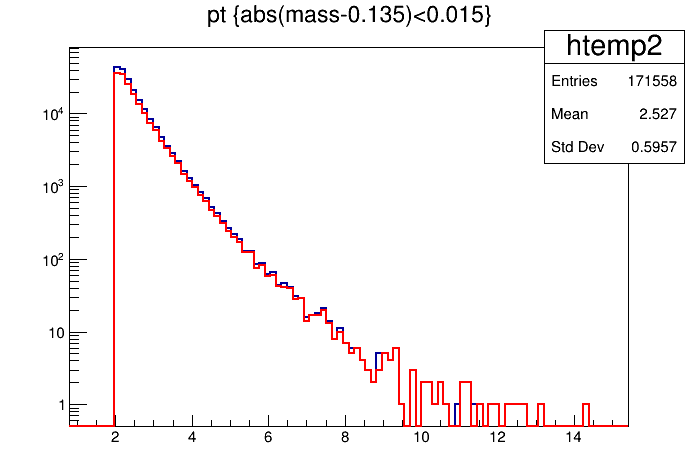
\includegraphics[width=0.45\linewidth]{figs/mbpi0pt.png}
  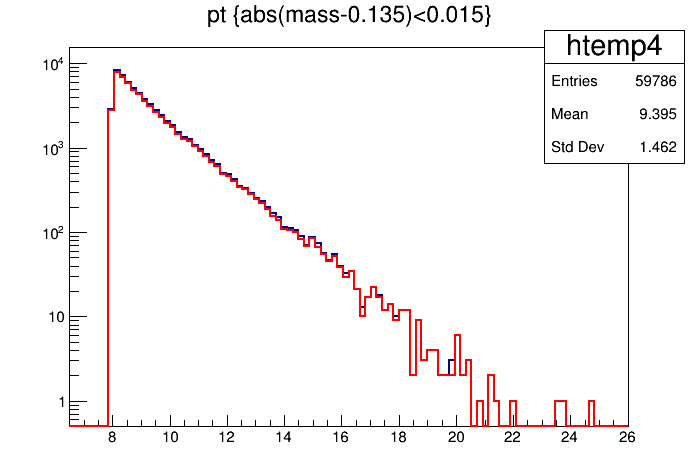
\includegraphics[width=0.45\linewidth]{figs/ertpi0pt.png}
  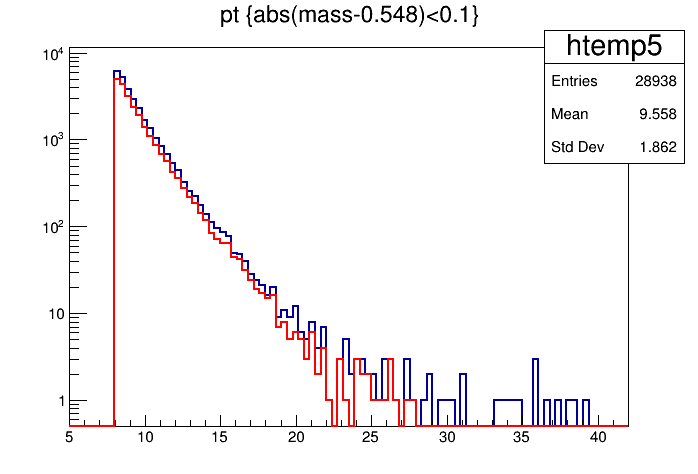
\includegraphics[width=0.45\linewidth]{figs/ertetapt.png}
  \caption{Transverse momentum (\pt) distributions of photon candidate
    pairs in the \piz window (top panels) and $\eta$ window (bottom
    panel).  Blue histograms: \pt for all pairs (no identification of
    the cluster as photon).  Red histograms: \pt for pairs where both
    clusters satisfy the {\it chisq} ``photonness'' criterion.
    Top left: MB data, top right and bottom: ERT data.
  }
    \label{fig:pizeta_pt}
\end{figure}
\end{center}

As stated earlier, the time-of-flight ({\it tof}) for clusters is
re-adjusted such that it will be zero for true photons.  In the left
panel of Fig.~\ref{fig:playtof} for cluster pairs which have an \mgg
in the \piz window we plot {\it tof} values vs each other.  True
\piz-s are in the big peak at (0,0).  If we now look at the horizontal
band to the right of the peak, the first cluster is still likely to be
a photon (small {\it tof}), but the second is more likely to be a
hadron.  Is this reflected in other observables characterizing the
clusters, too?  The answer is yes: on the right panel in
Fig.~\ref{fig:playtof} we plot the ``photonness'' variables 
{\it chisq1} in blue, {\it chisq2} in red.  The second cluster,
presumed hadronic, has on average higher {\it chisq2} value.

There is one more important lesson to be learned here.  Real-life
analyses are complicated.  There is no ``silver bullet'', single cut,
that, by miracle, selects {\it all} photons and nothing else.
Cuts are characterized by their {\it efficiency} (how much of the
desired signal they preserve) and {\it contamination} (how much of the
undesired signal passes).  Tighter cuts may reduce contamination, but
always at the cost of efficiency.  The art of analysis is to optimize
the signal/background, without sacrificing too much signal.
This is usually achieved by combining different cuts with AND or even
OR operations.  In the last decades probabilistic approaches of
combining cuts are also gaining ground.


\begin{verbatim}
ggntuple->Draw("tof1:tof2","abs(mass-0.135)<0.015&&abs(tof1)<20.0&&abs(tof2)<20.0","colz");
TH1D *hsmall = new TH1D("hsmall","hsmall",60,0.0,30.0);
TH1D *hlarge = new TH1D("hlarge","hlarge",60,0.0,30.0);
ggntuple->Draw("chisq1>>hsmall","abs(mass-0.135)<0.015&&abs(tof1)<3.0&&abs(tof2)>5.0");
ggntuple->Draw("chisq2>>hlarge","abs(mass-0.135)<0.015&&abs(tof1)<3.0&&abs(tof2)>5.0");
hlarge->SetLineColor(2);
hlarge->SetLineWidth(2);
hsmall->SetLineWidth(2);
hsmall->Draw();
hlarge->Draw("same");
\end{verbatim}

\begin{center}
\begin{figure}[htbp]
  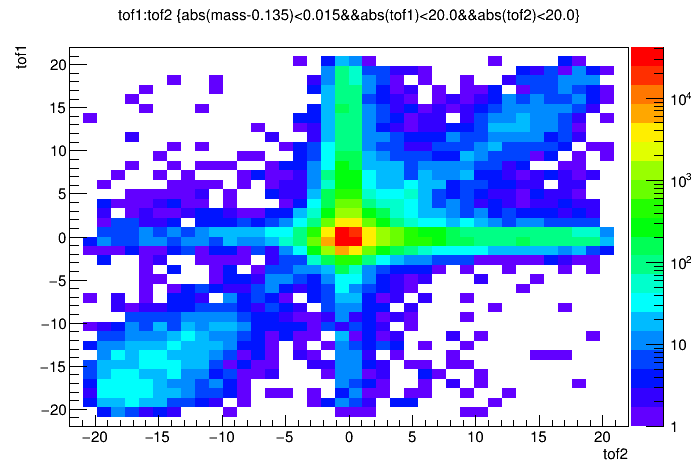
\includegraphics[width=0.45\linewidth]{figs/mbtof1tof2.png}
  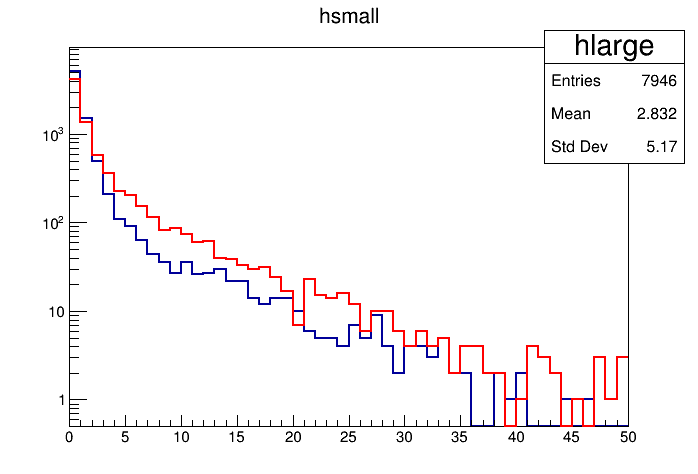
\includegraphics[width=0.45\linewidth]{figs/mbchi1chi2.png}
  \caption{Left panel: time-of-flight values of two clusters which
    produce an invariant mass in the \piz window.  TOF for true
    photons is per construction around zero so the true
    (non-combinatorial) pairs are in the sharp peak at (0,0).
    Right panel: {\it chisq} (``photonness'') of the clusters in the
    horizontal band above the main peak at (0,0).  Blue histogram is
    {\it chisq1} of the presumed true photon, the red histogram is the
    {\it chisq2} of the presumed hadron.  See text for more details.
  }
    \label{fig:playtof}
\end{figure}
\end{center}


Let's turn to single clusters (photon candidates, {\it gnt} Ntuple),
and look first at the position of the clusters (assumed impact point)
in a particular sector.  In Fig.~\ref{fig:deadhot} the $y,z$ positions
of the clusters are shown from MB and ERT data.  The depletion at the
edges is due to the algorithm (clusters too close to the edge are not
reconstructed because energy may leak out and the resulting 
{\it  ecore} will be incorrect).  The white areas represent ``dead''
channels that never fire, and the blue areas have only few hits,
although our expectation is that the clusters should be approximately
uniformly distributed over the sector.  Such dead or low-sensitivity
areas should be taken account in a real analysis when the acceptance
and efficiency of the detector are calculated.


\begin{verbatim}
f1->cd();
gnt->Draw("y:z","sec==1","colz");
f2->cd();
gnt->Draw("y:z","sec==1","colz");
\end{verbatim}


\begin{center}
\begin{figure}[htbp]
  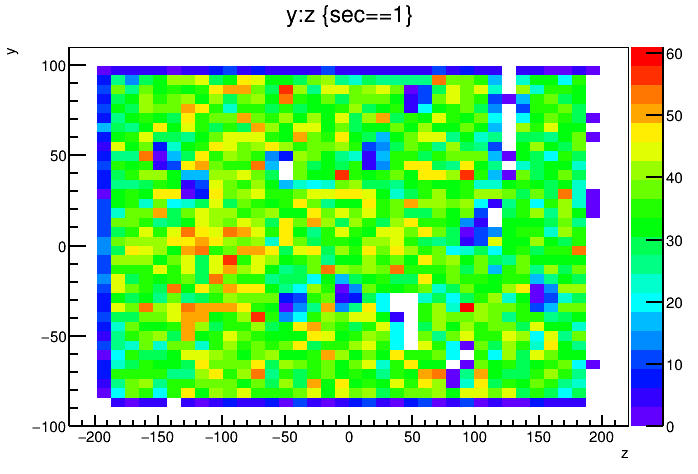
\includegraphics[width=0.4\linewidth]{figs/mbsec1_yz.png}
  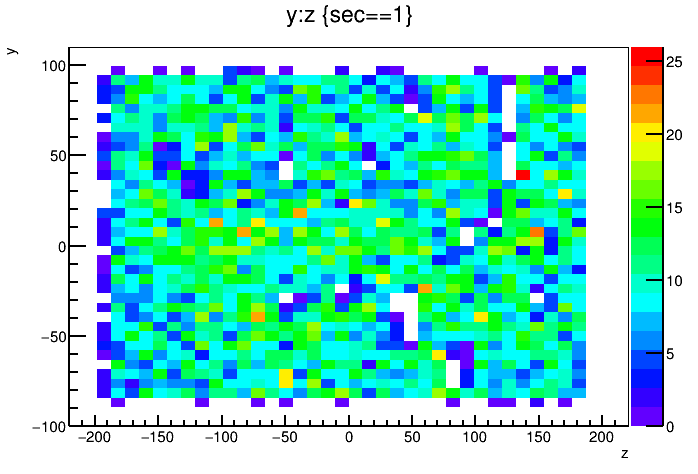
\includegraphics[width=0.4\linewidth]{figs/ertsec1_yz.png}
  \caption{Position of cluster centers (calculated impact point) in
    sector 1 (PbSc West).  Left panel: MB data.  Right panel: ERT data.
  }
    \label{fig:deadhot}
\end{figure}
\end{center}

Unfortunately not all clusters in {\it gnt} are photons.  The 
{\it chisq} variable is an estimate of the ``photonness'' based on a
parametrized shower profile, but its detailed description is beyond
the scope of this write-up.  However, it is interesting to look at the
compactness of the shower.  Electromagnetic showers are narrow, most
of the energy is deposited in a single tower, while
hadronic showers are fairly wide.  Besides the total energy 
({\it ecore}) the Ntuple also stores the energy in the ``central''
(most energetic) tower ({\it ecent}).  The ratio
{\it ecent/ecore} is expected to be high for photons, lower for
hadrons.  In Fig.~\ref{fig:ecentecore} this ratio is plotted versus
the total energy for MB data, first without any other cuts, then
cutting on the {\it chisq} variable, first deliberately selecting 
``photon-like'' showers, then ``un-photon-like'' showers.  Without
cuts the {\it ecent/ecore} has two characteristic peaks, which then
get almost perfectly resolved by the ``photon - not photon'' cut.  Of
course that also means that {\it ecent/ecore} in its own right can be
a powerful cut to select photons. 

\begin{verbatim}
f1->cd();
gnt->Draw("ecent/ecore:ecore","ecore<4.0","colz");
gnt->Draw("ecent/ecore:ecore","ecore<4.0&&chisq<3.0","colz");
gnt->Draw("ecent/ecore:ecore","ecore<4.0&&chisq>5.0","colz");
\end{verbatim}



\begin{center}
\begin{figure}[htbp]
  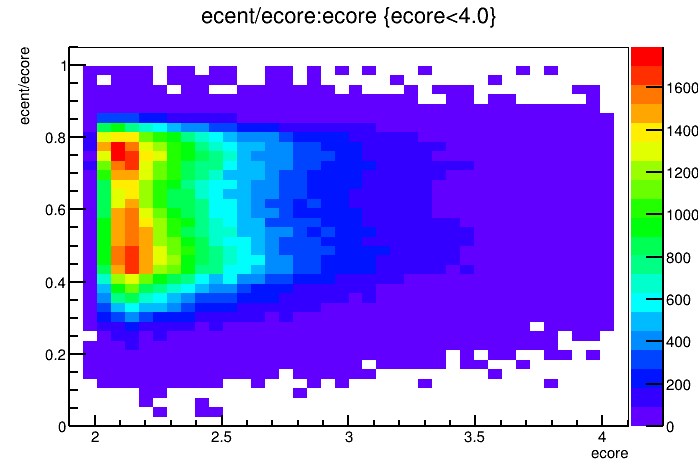
\includegraphics[width=0.3\linewidth]{figs/mbcentcore_nocut.png}
  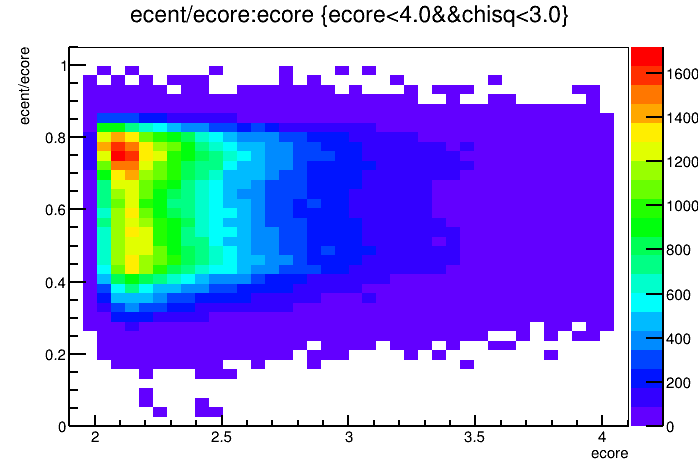
\includegraphics[width=0.3\linewidth]{figs/mbcentcore_chilt3.png}
  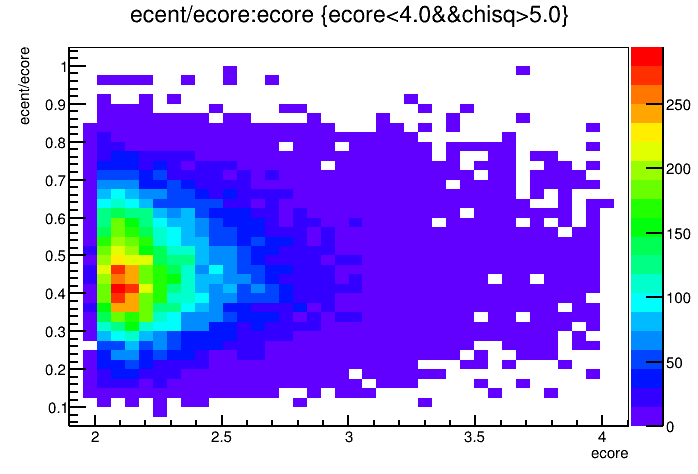
\includegraphics[width=0.3\linewidth]{figs/mbcentcore_chigt5.png}
  \caption{Shower compactness ({\it ecent/ecore}) vs shower energy in
    MB data.  Left panel: no cuts.  There is a characteristic
    double-peak structure.  Using the {\it chisq} (``photonness'')
    variable on the middle panel we select showers that are likely
    photons (small {\it chisq}), 
    on the right panel clusters that are most likely not
    photons (large {\it chisq}).  The compactness variable is quite powerful
    distinguishing between them (i.e. for photon identification).
  }
    \label{fig:ecentecore}
\end{figure}
\end{center}

As mentioned before, the {\it chisq} variable is a powerful tool to
enhance photons and reject hadrons in the sample.  In 
Fig.~\ref{fig:ertgntpt} we plot the \pt distribution of the clusters
in the ERT data sample, first with no cut (blue histogram), then with
a cut on {\it chisq} (red histogram).  Without the cut, the spectrum
spectrum ``flattens out'' at high \pt, which is non-physical.  The
effect of the cut becomes visible early on, and will be quite dramatic
above 15\,\gevc.  Up to about 25\,\gevc the red histogram shows the
expected power-law shape, above that it also flattens out.  You may
try to cut also on other {\it gnt} variables to get rid of the
nonphysical flat part of the red histogram.




\begin{verbatim}
TH1D *h1 = new TH1D("h1","h1",100,0.0,50.0);
TH1D *h2 = new TH1D("h2","h2",100,0.0,50.0);
h1->SetLineWidth(2.0);
h2->SetLineWidth(2.0);
h2->SetLineColor(2);
gnt->Draw("pt>>h1","");
gnt->Draw("pt>>h2","chisq<3.0");
h1->Draw();
h2->Draw("same");
\end{verbatim}


\begin{center}
\begin{figure}[htbp]
  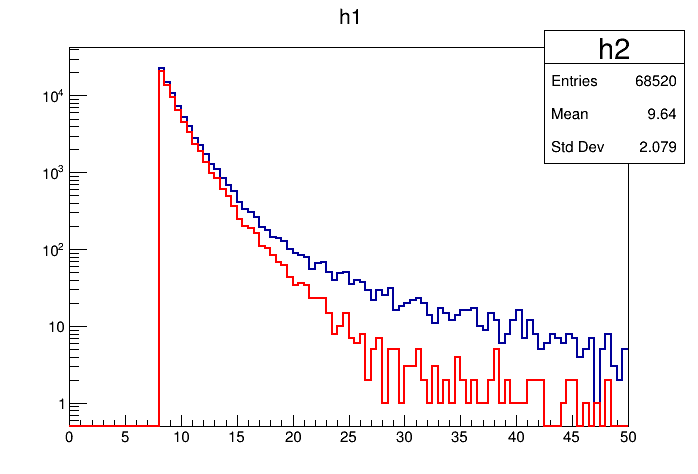
\includegraphics[width=0.5\linewidth]{figs/ertgntpt}
  \caption{Blue histogram: \pt spectrum from the ERT data, 
    {\it gnt} ntuple.  Red spectrum: same, but with a cut on
    ``photonness'' ({\it chisq}).  Much - albeit not all - of the
    nonphysical flattening at high \pt is gone.
  }
  \label{fig:ertgntpt}
\end{figure}
\end{center}


%\newpage
%\vspace{0.1in}
%{\bf Excercises} \\
%\vspace{0.05in}

%\noindent


\noindent
Please continue to play with the data!  The variables in the ntuples
are there for a reason!  Try plotting them against each other, making
them part of cuts when you plot a spectrum.  Make invariant mass plots
in bins of pair \pt, fit the combinatorial background with some simple
function (first, second order polynomial) and try to get a ``clean''
raw \piz yield as a function of \pt.  Try to imagine in advance, what
effect a cut would have, then actually make it and compare the result
with your expectations.  If you are open-minded and play creatively
with them, {\it the data will start speaking to you and telling you,
  how to analyze them}.

\vspace{0.2in}

\noindent
{\bf Have fun!}

%\begin{table}[h]
%  \begin{tabular}{|l|c|c|c|c|c|c|} \hline
%   Experiment   &  $\sqrt{s}$  &  method  &   $\eta$   &   $p_T$   &
%   Publications  & Comment \\ \hline \hline
%   R412 / CERN  ISR &  $pp$ 45, 53\,GeV  &  calor.  &
%   $|\eta|\sim 0$   &   1.6-3.8\,GeV/$c$   &
%   \cite{Darriulat:1976fb}  (1976) & $\gamma/\pi^0$ \\
%    ATLAS / CERN LHC  &  $pp$ 13 and 8\,TeV  &  calor.  &   $|\eta|<2.37$
%   &   125-1500\,GeV   &   \cite{Aaboud:2019vpz} (2019)  &
%   iso. $\sigma_{13}/\sigma_{8}$ \\ \hline
%  \end{tabular}
%  \vspace{0.3cm}
%  \caption{Summary of $pp$ and $p\bar{p}$ direct photon data (spectra,
%    cross-sections).
%}
%  \label{tab:ppdata}
% \end{table}
%


%\begin{center}
%\begin{figure}[htbp]
%  \includegraphics[width=0.5\linewidth]{figs/zdc_a470_fig1.pdf}
%  \caption{ZDC location between the beampipes, downstream after the DX
%    magnet $\pm$18\,m from the collision point.  (Figure taken 
%    from~\cite{Adler:2000bd}.)
%  }
%    \label{fig:zdc_a470_fig1}
%\end{figure}
%\end{center}


%\clearpage

%\bibliographystyle{unsrt}
%\bibliography{mpc_shortdoc}



\end{document}

